\chapter{WARP Graphs (WARP): Graphs All the Way Down}
\label{chap:warp-graphs-all-the-way-down}

Most people think of a graph as a drawing. Dots and lines. Boxes and arrows. Something you sketch on a whiteboard when the system gets too messy to hold in your head. It is a simplification tool, a way to tame complexity by drawing boundaries around it.

But a funny thing happens once you start using graphs to describe real systems:

\textbf{Your graphs get complicated. Very complicated.}

And then comes the inevitable, horrifying moment: The moment when the system you're modeling contains elements that are \textit{themselves} graphs.

Consider a build step. It isn't just a box labeled "Compile"; it produces multiple dependency graphs of artifacts. Consider a game entity. It isn't just a dot; it is composed of graphs of components, behaviors, and states. Consider a distributed system. Its services have internal dependency graphs, routing tables, and data flows.

A compiler turns syntax trees (graphs) into Intermediate Representation (graphs) into Control-Flow Graphs. An AI model is built from graph-shaped layers that operate on graph-shaped data. A simulation world is a place where every object, every constraint, every event is... yep. A graph.

Your graph now contains smaller graphs. Those smaller graphs contain graphs. And when you try to write it down, the hierarchy starts looking less like a network and more like a directory tree from hell:

\begin{lstlisting}[language=bash]
Graph
  ├─ Node
  │    └─ Graph
  │         ├─ Node
  │         └─ Node
  └─ Node
       └─ Graph
           └─ Node
\end{lstlisting}

At this point, the whiteboard marker squeaks. Someone in the room mutters, "oh no." Someone else quietly erases their earlier diagram, realizing it was woefully inadequate.

And you realize:

\begin{quote}
\textbf{The structure of your system isn't a graph. It's a graph of graphs. A recursive graph. A WARP graph.}
\end{quote}

Once you see this shape, you can't unsee it. It is the same pattern at every scale. Objects made of objects. Systems made of systems. Graphs made of graphs. Complex software piles structure inside structure until it stops resembling a diagram and starts resembling geology.

Layer after layer after layer. And if software is layers... then the only honest way to model it is with a structure that can express layers. That structure is the WARP Graph.

This is where the book really begins.

\section{The Moment the Diagrams Stop Being Diagrams}
\label{sec:diagrams-stop}

There's a moment in every engineer's life when the diagrams stop being diagrams. It usually happens around hour three of a debugging session. You're sketching a pipeline, trying to understand how some piece of the system went sideways, and you realize your whiteboard looks less like an architecture diagram and more like the stratigraphy of a planet.

Layers on layers. Systems inside systems. Graphs inside graphs.

You zoom in on one part of the system and find more structure. Zoom in again—more structure. Zoom in again—still more. At some point, a teammate walks past, glances at your diagram, and asks: "Dude... is that a graph inside an edge of another graph?"

And you look down at the board and say: "Uh... yeah. Actually... yeah. It is."

Welcome to WARP Graphs—the moment you realize the system wasn't a flat graph at all. It was graphs all the way down.

\section{Why Ordinary Graphs Break at Scale}
\label{sec:graphs-break}

Most systems start simple. You draw boxes for components, arrows for communication, and everything feels sane. But complexity has a way of hiding in plain sight.

\begin{itemize}
    \item The "renderer" turns out to be a graph of passes and stages.
    \item The "physics engine" turns out to be a graph of solvers and constraints.
    \item The "AI system" turns out to be a graph of behavior trees and decision nodes.
    \item The "networking layer" turns out to be a graph of protocols and handshakes.
    \item The "compiler" turns out to be a graph of graphs of graphs.
    \item The "microservice" turns out to have five internal DAGs handling requests.
    \item The "build step" turns out to be an entire universe of dependencies.
\end{itemize}

Everything that looked like a node turns out to contain... more graphs. And everything that looked like an edge turns out to contain... more system.

This is not an abstraction failure. This is how complexity behaves. Complex systems compose recursively, not linearly.

\section{The First Realization: Nodes Contain Structure}
\label{sec:nodes-contain-structure}

The simpler revelation—the one people see first—is that a node in a real system is NOT atomic. It is a container of structure.

A "physics engine" node contains a broadphase graph, a narrowphase graph, a constraint graph, and an integration graph. A "compiler step" node contains an AST, an IR, a CFG, and an optimization graph. A "microservice" node contains routing graphs, dependency graphs, storage graphs, and event graphs.

Every real node is secretly a meta-node—a graph in disguise. This is the first hint that WARP graphs are necessary. But then it gets deeper. Much deeper.

\section{The Bigger Realization: Edges Contain Structure Too}
\label{sec:edges-contain-structure}

Most diagrams lie by treating edges as thin arrows. In real systems, edges are not arrows. \textbf{Edges are processes.}

Edges have protocols, timing, buffering, constraints, state, retries, invariants, sub-flows, pipelines, logic, and transformations.

A "simple edge" like $A \rightarrow B$ might represent:
\begin{itemize}
    \item An HTTP request with headers, body, and timeout logic.
    \item A shader compile pass with multiple stages.
    \item A physics constraint resolving forces over time.
    \item An AI decision traversing a logic tree.
    \item An RPC with retry policies and circuit breakers.
    \item A transactional update with rollback capabilities.
\end{itemize}

In every case, the edge has its own internal structure. Usually a whole graph.

So... if nodes can contain graphs... and edges can also contain graphs... then what you're modeling isn't a graph. It's a \textbf{WARP Graph}.

\begin{figure}[h]
    \centering
    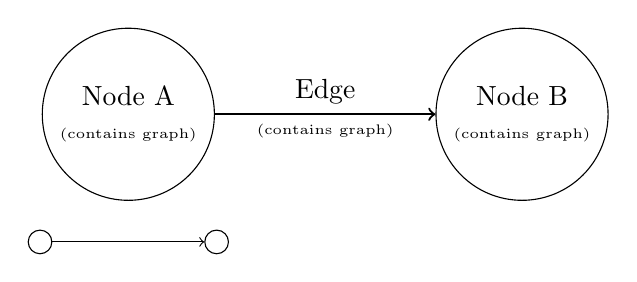
\begin{tikzpicture}[node distance=3cm, auto]
        % Outer Graph
        \node (A) [draw, circle, minimum size=1.5cm, align=center] {Node A \\ \tiny(contains graph)};
        \node (B) [draw, circle, minimum size=1.5cm, align=center, right of=A, node distance=5cm] {Node B \\ \tiny(contains graph)};
        
        % Edge as a container
        \draw[->, thick] (A) -- node[above] {Edge} node[below] {\tiny(contains graph)} (B);
        
        % Inner Graph for Node A (conceptual visualization)
        \node (subA1) [draw, circle, inner sep=1pt, minimum size=0.3cm, below left of=A, xshift=1cm, yshift=0.5cm, fill=white] {};
        \node (subA2) [draw, circle, inner sep=1pt, minimum size=0.3cm, below right of=A, xshift=-1cm, yshift=0.5cm, fill=white] {};
        \draw[->, thin] (subA1) -- (subA2);
        
    \end{tikzpicture}
\caption{Visualizing a WARP graph: Nodes and edges are containers for deeper structure.}
    \label{fig:rmg_concept}
\end{figure}

\section{WARP Graphs: The True Shape of Complex Software}
\label{sec:rmg-definition}

Here's the clean definition in human language:

\begin{quote}
\textbf{A WARP graph is a graph where nodes may contain WARP graphs and edges may contain WARP graphs.}
\end{quote}

That's it. Simple idea, enormous consequences. This structure is fractal, self-similar, infinitely nestable, compositional, multi-scale, multi-domain, and recursively expressive.

\textbf{WARP graphs are what complex systems actually look like.} Ordinary graphs are the cartoon version. WARP graphs are what you get once you take off the training wheels.

\section{Edges as Wormholes: The Intuition That Finally Makes Sense}
\label{sec:edges-wormholes}

This is the moment your brain stops fighting the structure and starts cooperating. In a WARP, an edge is not a line. It is a \textbf{wormhole}.

NOT a sci-fi "walk in and teleport unchanged" wormhole. That metaphor is wrong. The correct metaphor is a wormhole that \textit{transforms} you. You enter as \texttt{Foo} and exit as \texttt{Bar}.

These are wormholes:
\begin{itemize}
    \item Compilers
    \item Shader pipelines
    \item Database query planners
    \item Neural nets
    \item Registries
    \item Render pipelines
    \item Solver iterations
    \item Distributed protocols
    \item Serialization/deserialization logic
    \item Build steps
\end{itemize}

These aren't "arrows." They are \textit{tunnels of computation with internal geometry}. Edges are not conduits. Edges are \textit{processes}. Edges don't transport. Edges \textit{rewrite}.

\begin{tcolorbox}[colback=gray!10, colframe=black, title=\textbf{📦 FOR THE NERDS™: Formal Shape of a WARP graph}]
We model a WARP graph as a tuple:
\[ WARP = (V, E, subV, subE) \]
where:
\begin{itemize}
    \item $V$ — the set of nodes
    \item $E \subseteq V \times V$ — the set of edges
    \item $subV: V \rightarrow WARP \cup \{\emptyset\}$ — recursively nested node content
    \item $subE: E \rightarrow WARP \cup \{\emptyset\}$ — recursively nested edge content
\end{itemize}

\textit{This recursive closure makes WARP graphs coalgebras of a graph functor.}

\textbf{Edges and nodes are equal citizens.}
\end{tcolorbox}

\section{The Compiler: A Wormhole in Disguise}
\label{sec:compiler-wormhole}

Let's illustrate the idea with the cleanest example in software: the Compiler.

\[ [\text{Source Code}] \xrightarrow{\text{Compiler Wormhole}} [\text{Machine Code}] \]

Inside that single edge lies a massive universe: Lexing, Parsing, AST construction, IR generation, Control Flow Graphs, SSA conversion, optimization passes, register allocation, and code generation.

In a flat graph, this is impossible to model without exploding the diagram into unreadability. In a WARP graph, it is natural. Nodes model \textit{state}. Edges model \textit{transformation universes}.

\section{Why WARP Graphs Matter (Spoiler: DPO)}
\label{sec:rmg-matter}

WARP graphs give us multi-scale structure, nested universes, structured transformations, rewrite surfaces, rule-scoped regions, compositional boundaries, context for evolution, and geometry for comparing worlds.

But they also give us something much more important:

\textbf{\textit{A substrate where rewrite rules can operate anywhere.}}

This is what \textbf{Chapter 4} is about. \textbf{Double-Pushout (DPO) rewriting is the physics of WARP graphs.}

And because nodes and edges can contain WARP graphs, DPO rules can match and rewrite whole worlds, subworlds, transitions, pipelines, logic, flows, clauses, constraints, states, and histories. DPO is not an add-on. It's the rule of rules.

\section*{Transition: From Structure to Motion}

We've spent three chapters describing structure:
\begin{enumerate}
    \item Flows (\textbf{Chapter 1})
    \item Graphs (\textbf{Chapter 2})
    \item Recursive Universes (\textbf{Chapter 3})
\end{enumerate}

Structure alone doesn't compute. Structure alone doesn't evolve. Structure alone doesn't create possibility. For that, we need \textbf{rules}.

The things that cause change, evolve state, split universes, merge universes, define adjacency, distance, paths, and worldlines.

This leads directly to:

\textbf{$\rightarrow$ Chapter 4 — Double-Pushout Physics (DPO): The Rule of Rules}

\textit{Where edges-as-wormholes gain laws, WARP graphs begin to move, and computation becomes geometry.}
